\lhead{Arquitectura física}
\chapter{Arquitectura física}

\section{Introducción}

El sistema a crear, si bien de carácter distribuido, localiza el conjunto de nodos principales en una misma ubicación física, externalizando únicamente los componentes secundarios.

Esta centralización apoya uno de los objetivos principales del proyecto. Al contar con todo el sistema en una única ubicación es posible comprender mejor los mecanismos de distribución de tareas de forma más efectiva que en un sistema distribuido por toda la infraestructura. Esta decisión aporta además una serie de ventajas técnicas, entre las que figuran las siguientes:

\begin{itemize}
\item Centralización del sistema de alimentación eléctrica.
\item Reducción del cableado de red.
\item Favorece la organización de todos los componentes del sistema.
\item Facilita el traslado del sistema a otra ubicación.
\item Simplifica el mantenimiento del sistema.
\end{itemize}

\section{Requisitos}

\subsection{Coste}

El coste de la estructura debe reducirse al máximo sin que esto comprometa el resultado final.

\section{Propuestas de solución}

A fin de minimizar el coste, se buscan soluciones que permitan ahorrar en el coste final.

\subsection{Primera propuesta}

En las primeras fases del proyecto se plantea la utilización de separadores de nylon atornillados a los orificios que las placas disponen para tal fin, creando una pequeña estructura en forma de torre. Dicha solución se acepta debido a su efectividad con un precio bajo.

\subsection{Segunda propuesta}

La segunda propuesta apuesta por mejorar la versatilidad del diseño. Se plantea un diseño en forma de estantería que incluya una bahía para cada nodo, permitiendo la extracción de cada uno de ellos de forma independiente, así como la instalación de nuevos nodos. Se decide desestimar el primer prototipo en pro de esta solución.

\subsubsection{Elección de materiales}

Inicialmente se valora el uso de metal para la construcción del esqueleto de la estructura, sin embargo finalmente se opta por el metacrilato como material, pues mejora la visualización de cada uno de los nodos y añade un mayor atractivo estético al proyecto.

Se utilizará latón como material de unión entre los diferentes componentes de metacrilato, utilizando tornillos a menos que estos deterioren la estética de la estructura, en cuyo caso se utilizarán adhesivos.

\subsubsection{Construcción}

La fase de construcción se extiende durante aproximadamente dos semanas (junto con el resto de tareas de desarrollo. El tiempo de desarrollo asciende a 20 horas).

\begin{figure}[H]
\centering
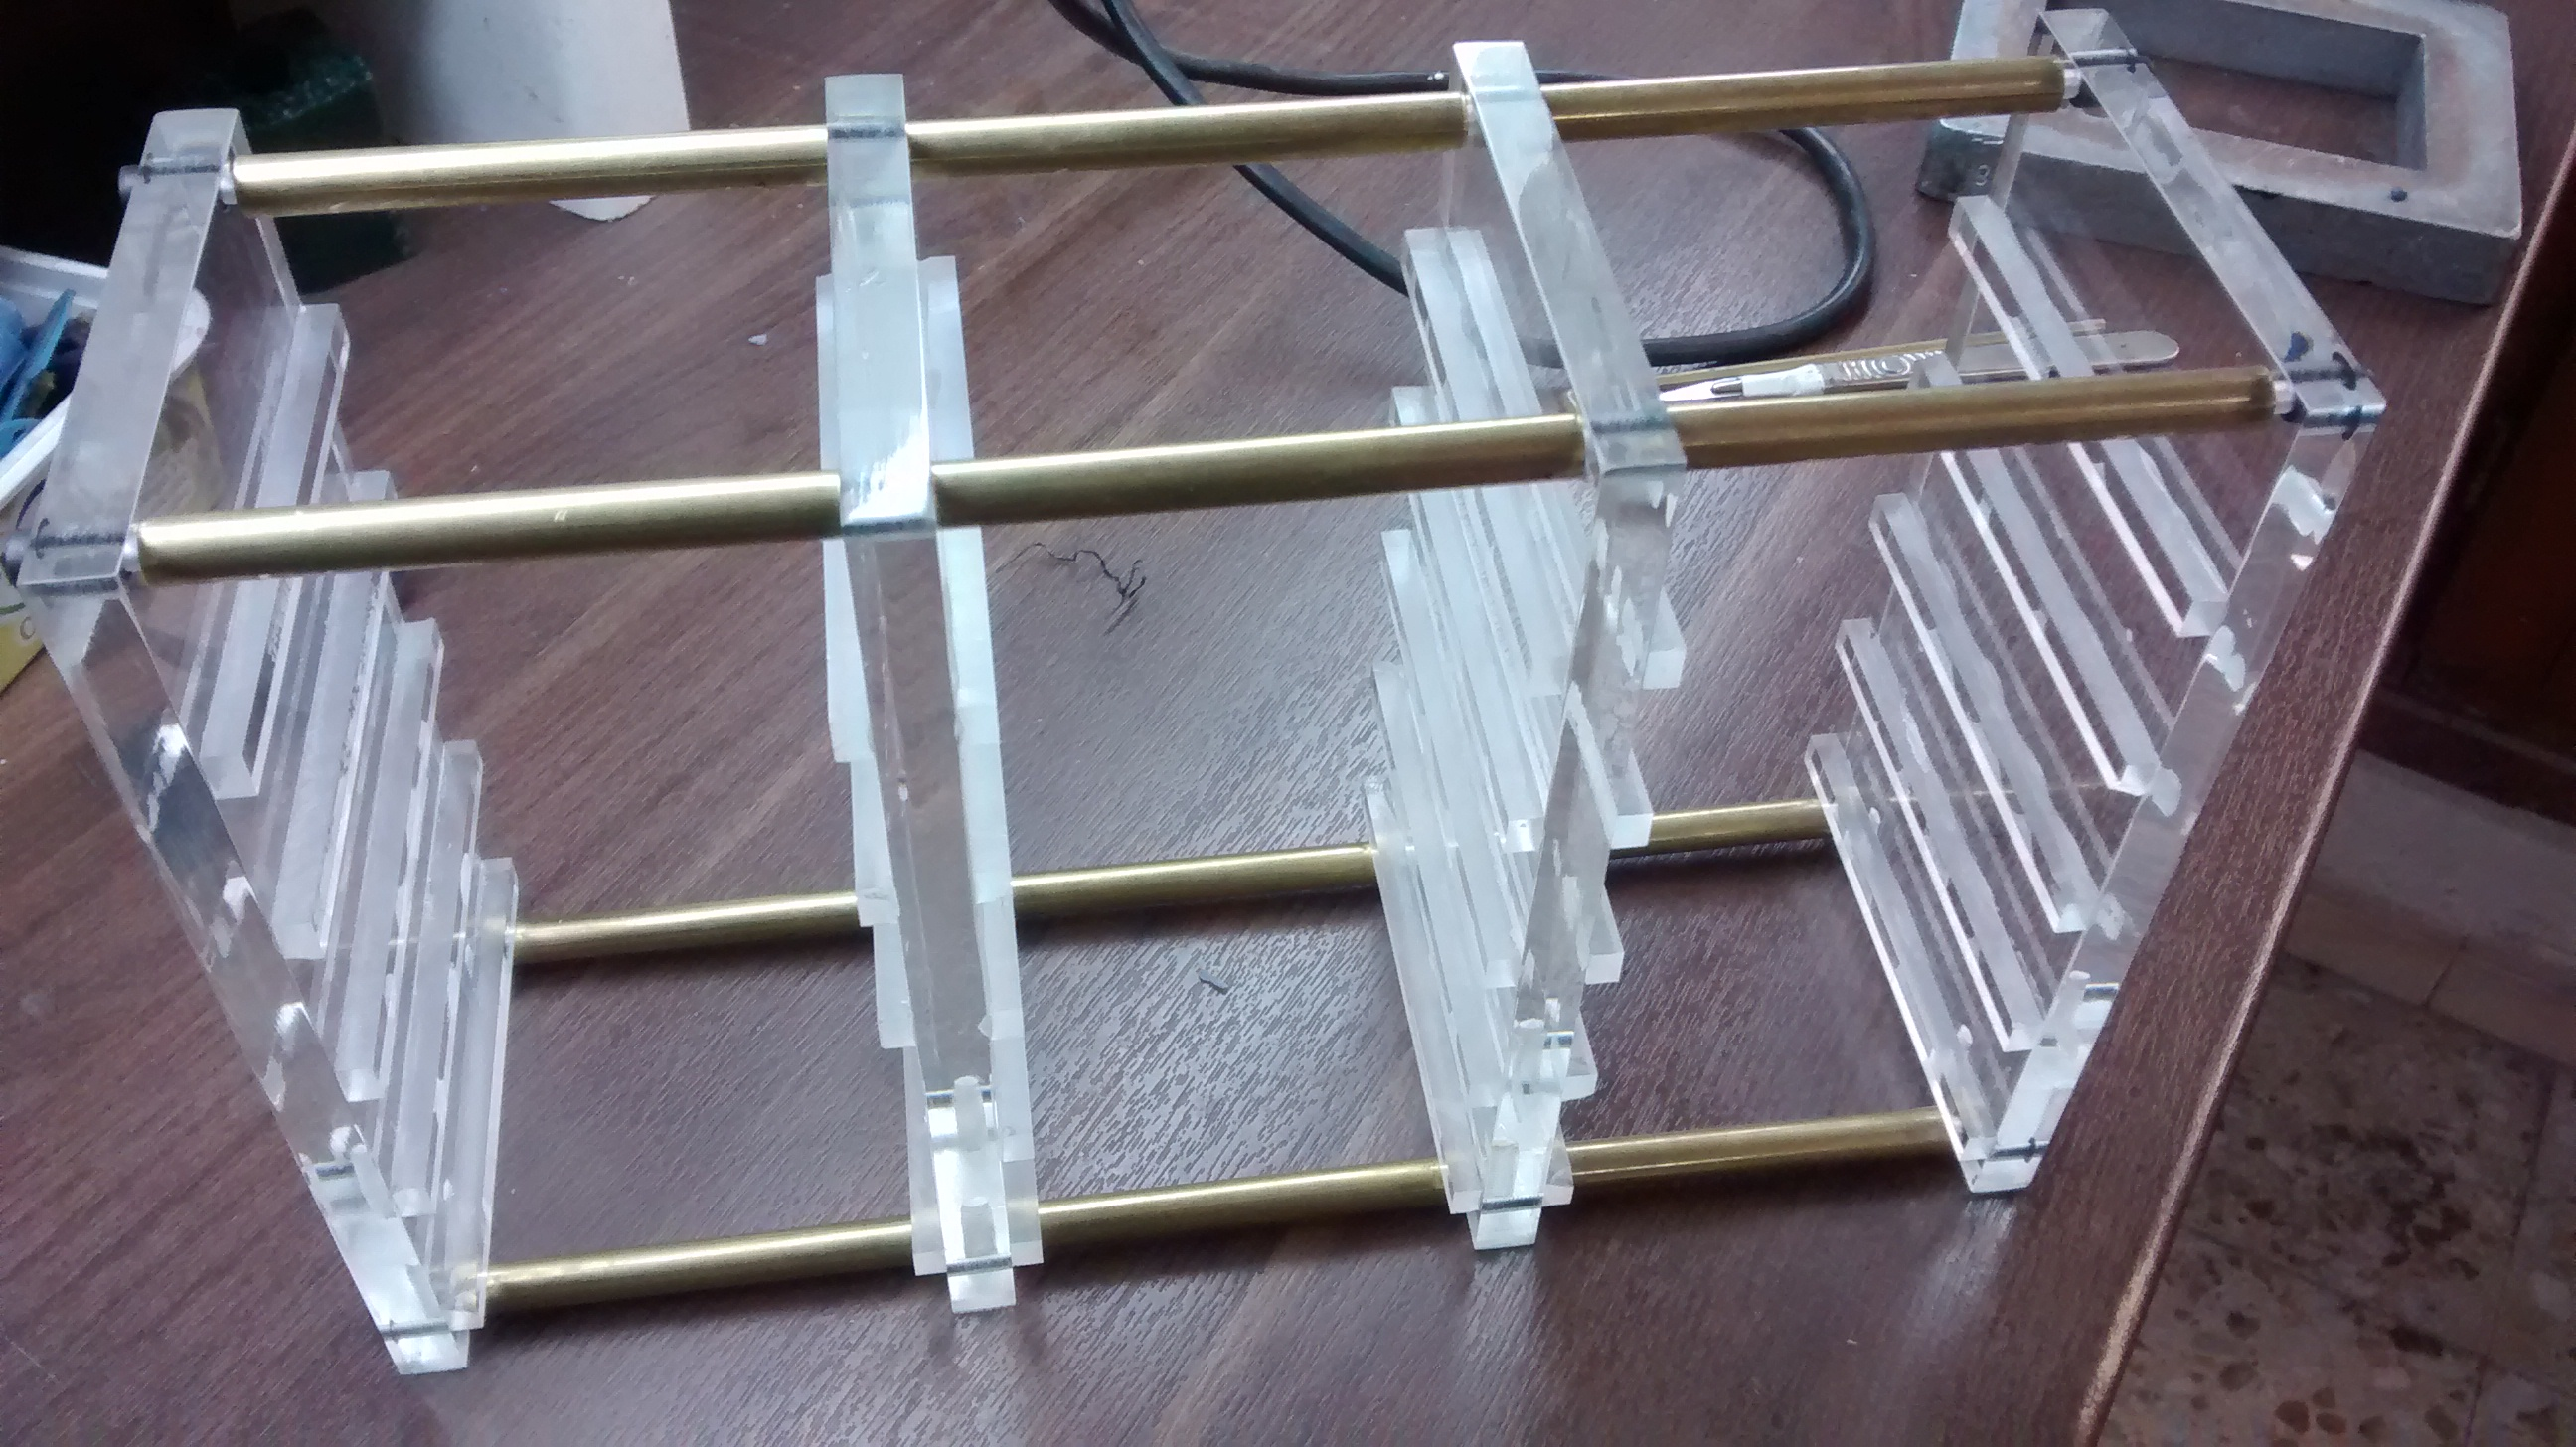
\includegraphics[width=0.635\textwidth]{Chapter5/Figures/prototipo1vistageneral}
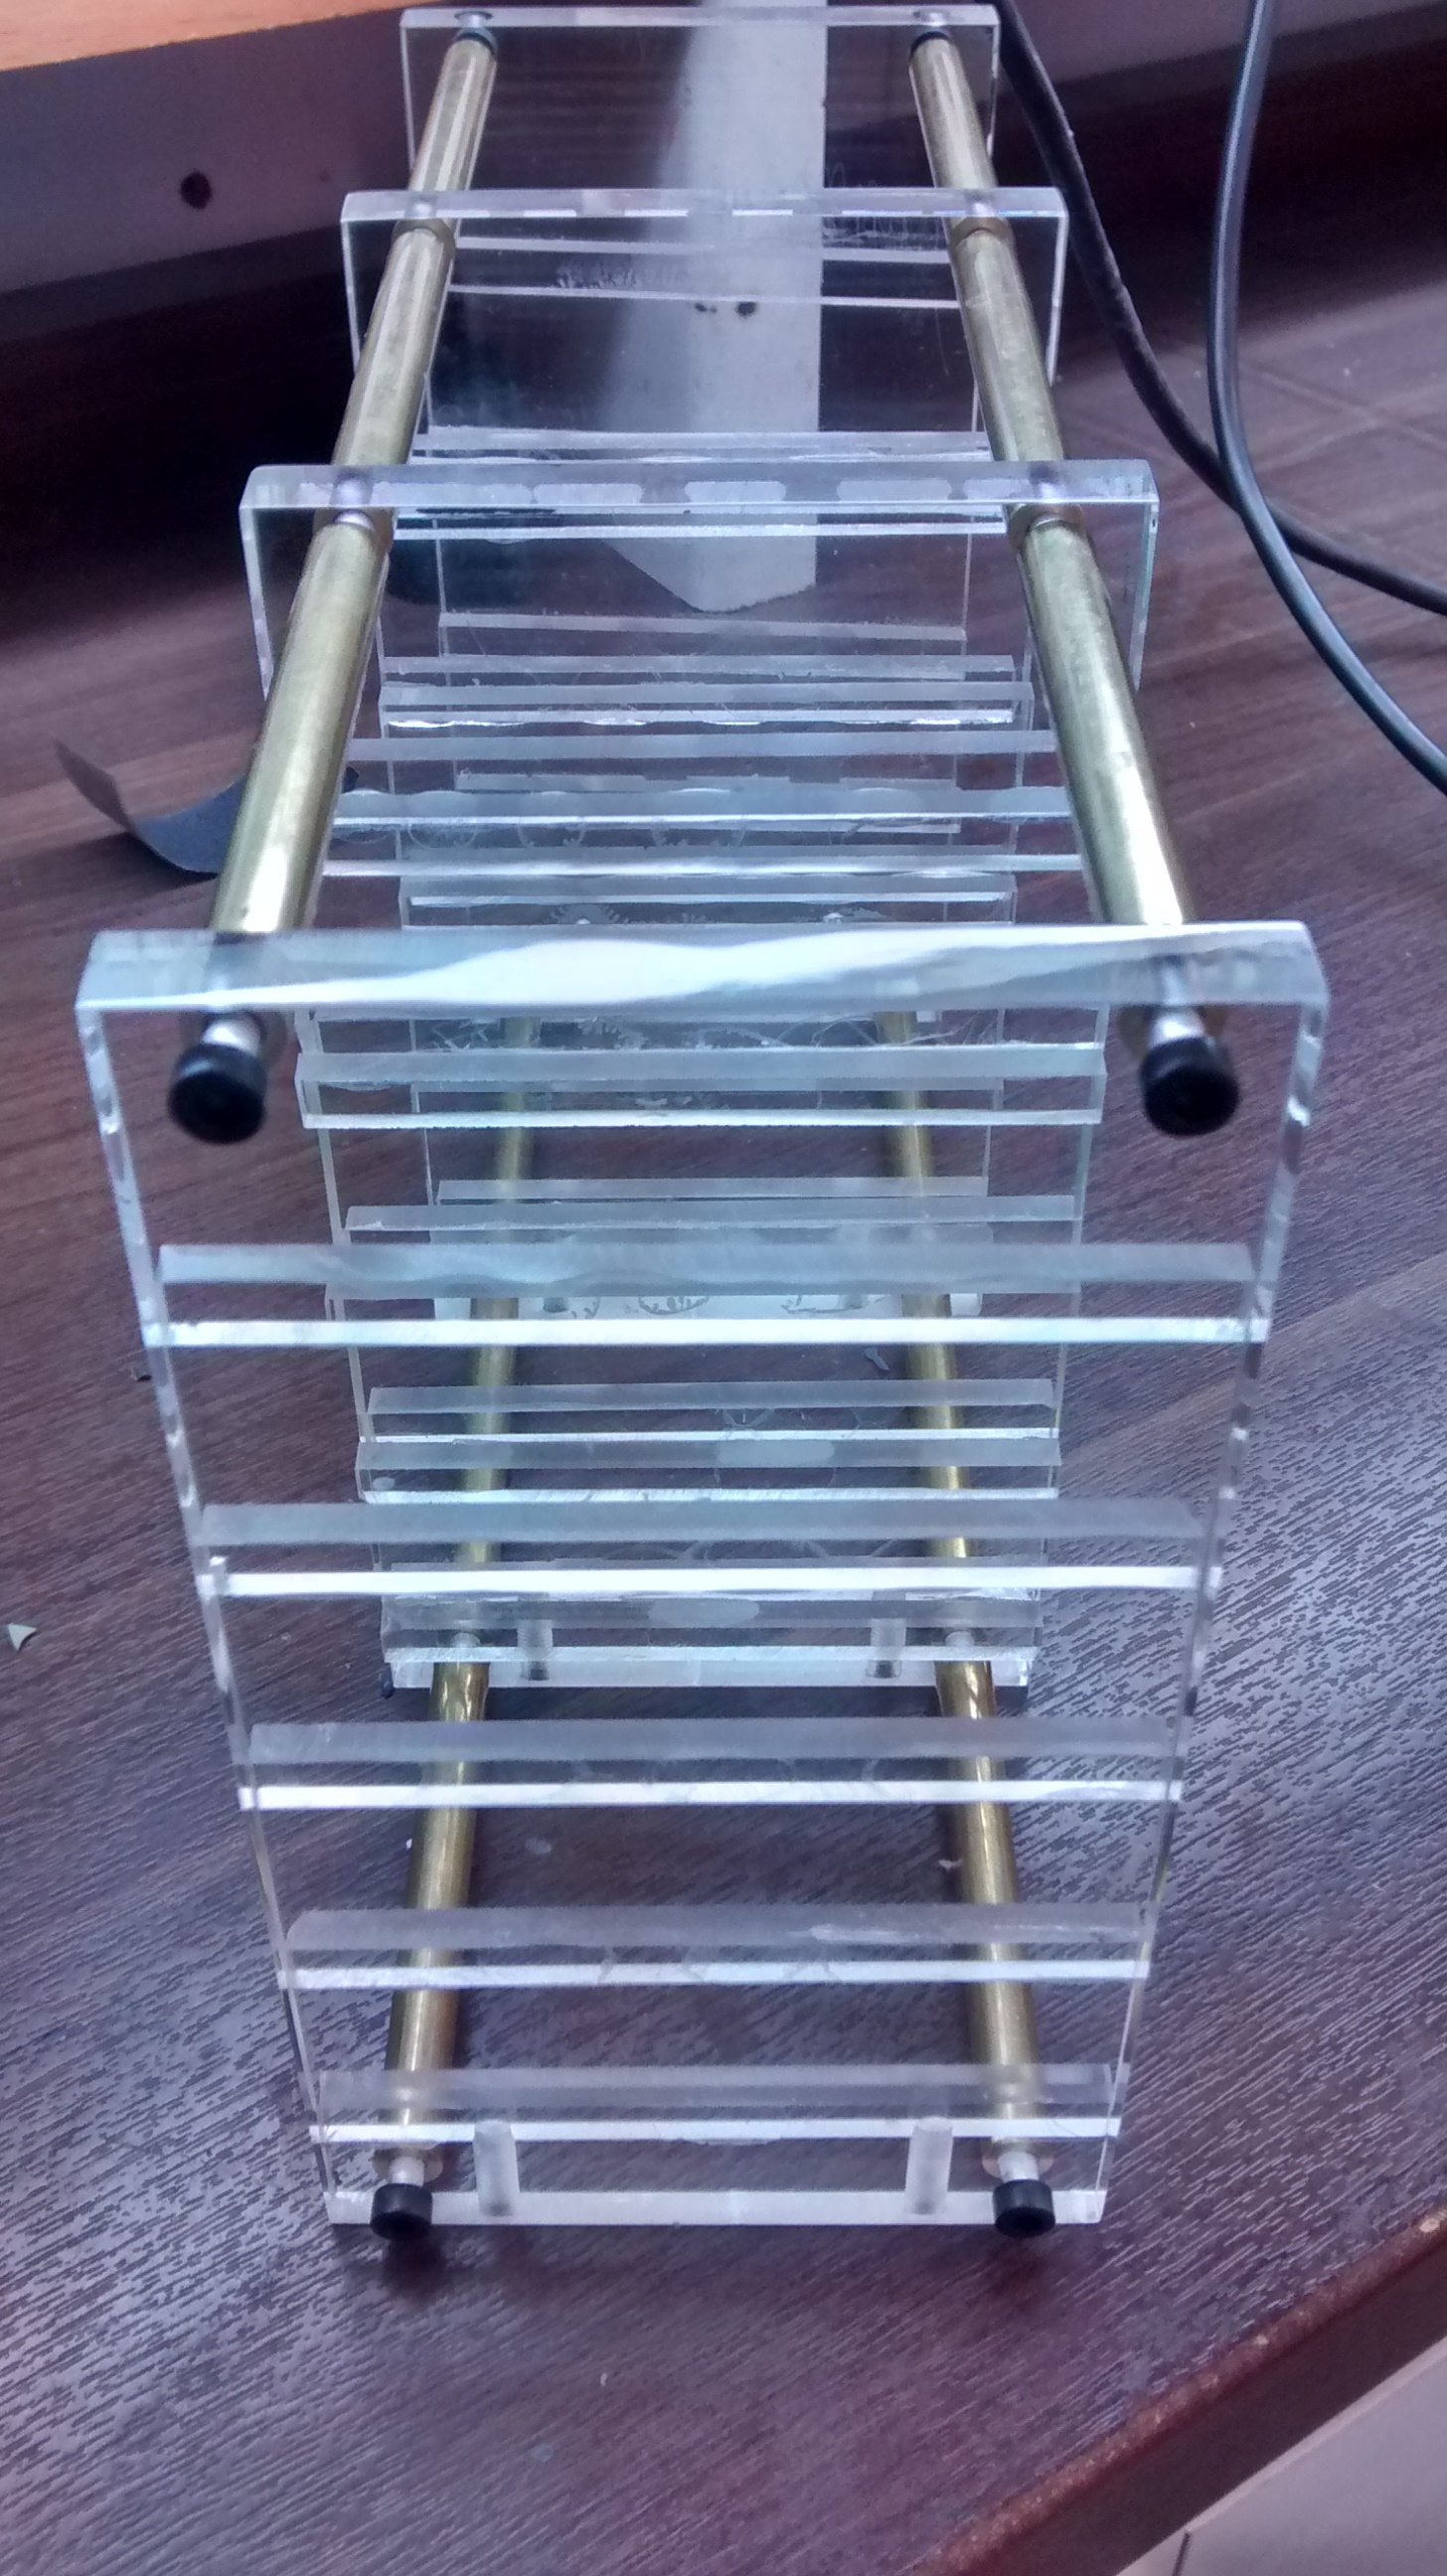
\includegraphics[width=0.2\textwidth]{Chapter5/Figures/prototipo1vistaperfil}
\caption[Vista general del primer prototipo]{Vista general de la estructura del primer prototipo y vista de perfil del mismo.}
\end{figure}

\begin{figure}[H]
\centering
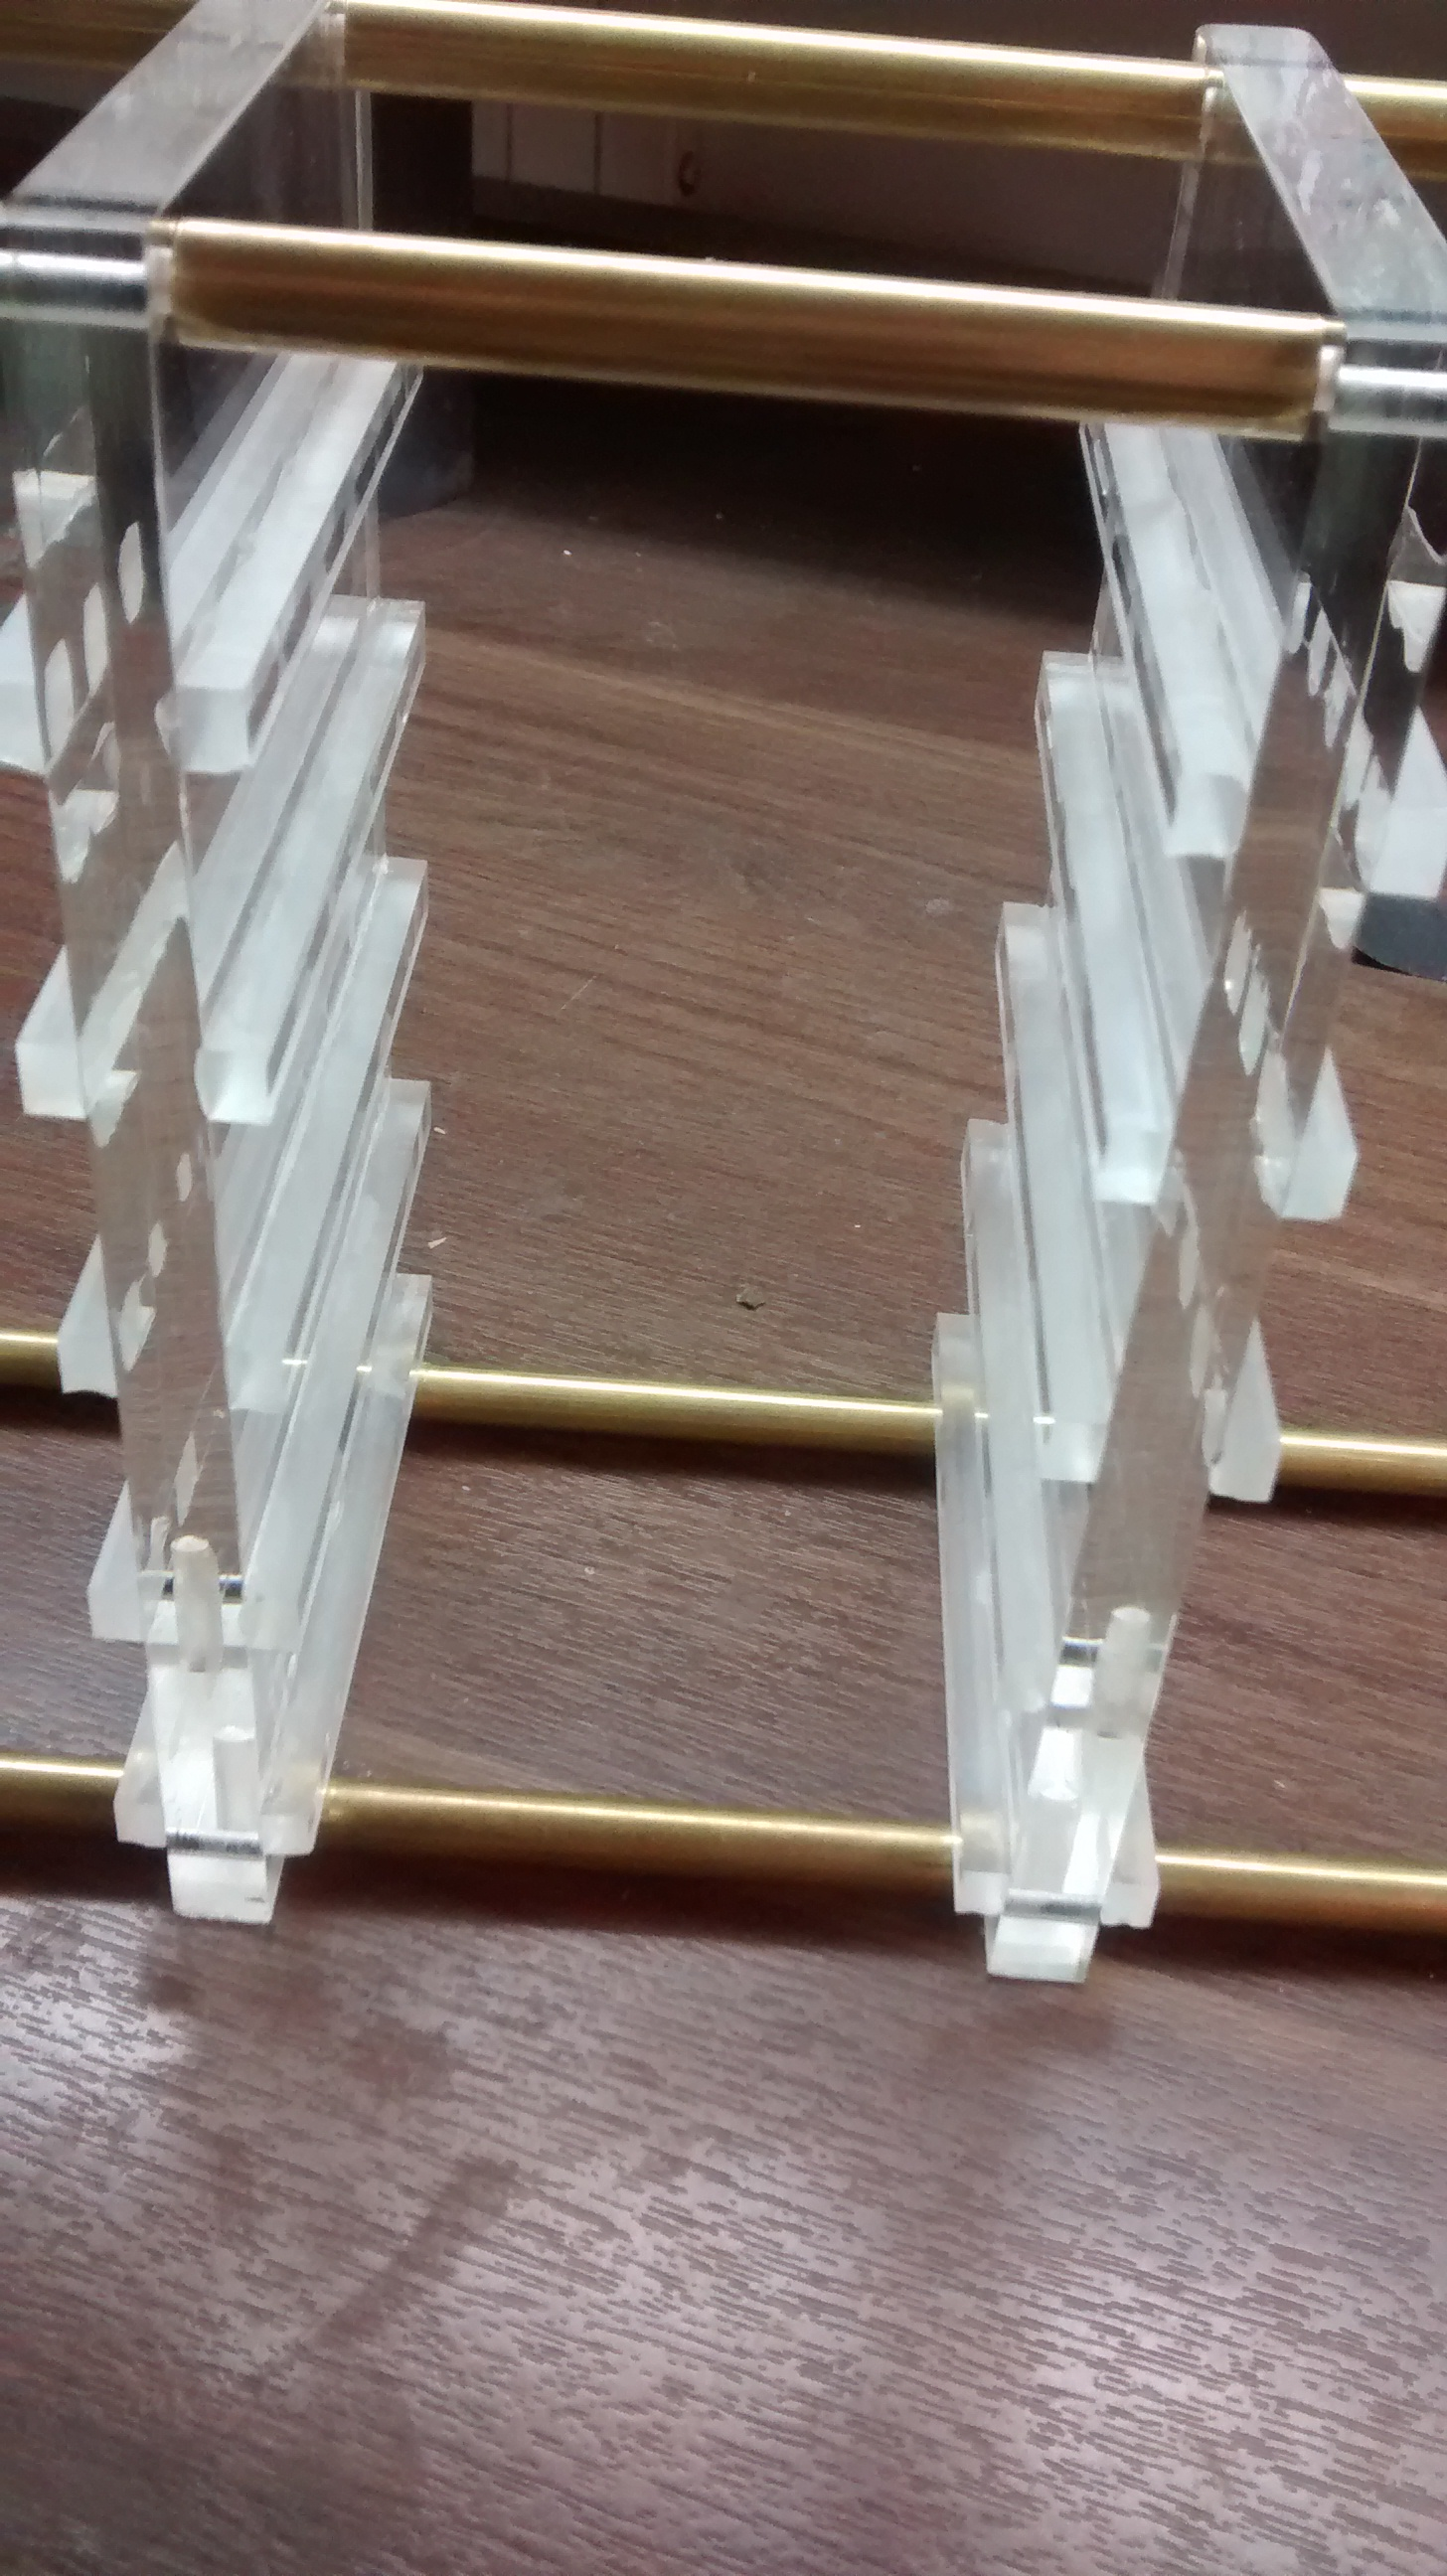
\includegraphics[width=0.2\textwidth]{Chapter5/Figures/prototipo1vistadetalle}
\caption[Vista en detalle de los ``raíles'' del primer prototipo.]{Vista en detalle de los ``raíles'' creados para cada uno de los nodos.}
\end{figure}

Este prototipo es considerado aceptable, y se decide partir del mismo para elaborar la solución final.

\subsection{Tercera propuesta}

A pesar del éxito del segundo prototipo, durante las siguientes fases de desarrollo se plantea la viabilidad del prototipo para albergar una serie de componentes que acompañen a los nodos. Utilizar, como se planteaba, un ladrón USB %TODO
para la alimentación del sistema parece una solución poco efectiva (incrementa la cantidad de cableado a utilizar). La conexión a la red también genera incertidumbre, pues se planteaba inicialmente la conexión a la misma de forma individual para cada nodo. Esta decisión complicaría la gestión del cableado.

Además, se observan errores en las medidas iniciales para cada uno de los raíles, pues no se contó con el espacio que los conjuntos de diodos LED consumirían.

Por ello, se plantea la elaboración de un tercer prototipo basado en el anterior que tenga las siguientes propiedades:

\begin{itemize}

\item La estructura albergará a todos los nodos así como los diferentes componentes que estos requieran para su funcionamiento.

\item El sistema deberá centralizar en un único mecanismo de alimentación el suministro de energía eléctrica a los nodos y a cualquier otro componente integrado en la estructura.

\item La conexión a la red de datos deberá estar centralizada.

\end{itemize}

\subsubsection{Elección de materiales}

Se mantienen las decisiones de materiales realizadas para el segundo prototipo, y se intentará reutilizar todo el material posible del mismo.

Para la alimentación eléctrica se decide utilizar una fuente de alimentación de 5 V capaz de suministrar hasta 100 W de energía permitiendo la conexión a la red eléctrica presente en la infraestructura.

Las conexiones de red se centralizarán en un switch con velocidades de hasta 100 Mb/s paralelos.

Sin embargo, queda aún una incógnita por resolver: si bien la fuente de alimentación es capaz de suministrar energía a los nodos, es necesario definir cómo se suministrará dicha energía. Se plantean dos opciones:

\paragraph{Alimentación a través del puerto GPIO\\}

El puerto \textbf{GPIO} de la Raspberry Pi es utilizado comúnmente para la alimentación de periféricos conectados a la misma, a través de varios pines dispuestos para tal fin. Sin embargo, es posible alimentar a la propia placa a través de los mismos\footnote{Esquema completo del circuito de la Raspberry Pi: \href{https://www.raspberrypi.org/wp-content/uploads/2012/04/Raspberry-Pi-Schematics-R1.0.pdf}{https://www.raspberrypi.org/wp-content/uploads/2012/04/Raspberry-Pi-Schematics-R1.0.pdf}}.%TODO[http://raspberrypi.stackexchange.com/questions/1617/how-do-i-supply-power-through-the-gpio]. 



Extendiendo dos cable desde la fuente de alimentación hasta los pines 1 y 3 (+5V y neutro) es posible alimentar la placa.

Sin embargo dicha solución implica un riesgo considerable, al no disponer el puerto GPIO de una serie de mecanismos de protección ante un uso como este (en el caso de la alimentación por USB se cuenta con dicha protección). En caso de una sobrecarga eléctrica la placa sería dañada de forma irreversible. Se plantea el uso de fusibles de 2 amperios para proteger a las placas de este tipo de sobrecargas.

\paragraph{Alimentación a través del puerto USB\\}

Es posible adaptar la propuesta de solución anterior a una alternativa más prometedora. Aprovechando los mecanismos de protección frente a sobrecargas del puerto USB se decide adquirir y modificar cabezas micro-USB macho para soldarlas a cables conectados a la fuente de alimentación. Dichas cabezas se conectarán a cada una de las placas. Se mantienen no obstante los fusibles ya adquiridos como medida preventiva conectando uno a cada cable de corriente positiva.

Esta solución permite centralizar todos los cables de alimentación en un único punto a la vez que se mantienen los mecanismos de protección que integran las placas, manteniendo a efectos prácticos el sistema de alimentación que se ideó para la Raspberry Pi.

Gestión de la red:

Se crearán cables ethernet a medida para cada uno de los raíles.

LEDs

Situar los diodos supone un problema significativo. Utilizar cualquier tipo de cableado complicaría el diseño de forma significativa, por lo que es necesario buscar una alternativa.

Como solución se decide crear placas con circuitos impresos que conecten los diferentes diodos al puerto GPIO, utilizando una tira GPIO soldada al circuito que se conectará a los pines de la Raspberry. De esta forma se evita cualquier tipo de cableado y se evita realizar soldaduras a la placa.

A fin de ahorrar espacio, los LED se situarán sobre la Raspberry cubriendo la parte inferior de la misma.

\section{Coste}

\begin{table}[H]
\centering
\begin{tabular}{|l|r|r|r|}
\hline
\textbf{Ítem} & \textbf{Unidades} & \textbf{Precio unitario} & \textbf{Total} \\ \hline
Placas de metacrilato de 10mm & 1 m\textsuperscript{2} & 1 & 30 € \\ \hline
Placas de metacrilato de 5mm & 1 m\textsuperscript{2} & 1 & 10 € \\ \hline
Placa de metacrilato de 4mm & 1 m\textsuperscript{2} & 1 & 20 € \\ \hline
Varilla de latón de 8mm & 1 & 1& 15 €\\ \hline
Tornillos & & & 10 €\\ \hline
Cable Ethernet & 3 metros & 1.2 €/metro & 3.6€\\ \hline
Fusibles de 2 A & 10 & 0.3 € & 3.15\\ \hline
Portafusibles & 12 & 0.5 & 6 € \\ \hline
Fuente de alimentación de 5 V & 1 & 16.63 & 16.63 \\ \hline
Tira de pines GPIO & 3 & 0.9 & 2.84 \\ \hline
Diodos LED & 24 & &\\ \hline
\end{tabular}
\caption{Coste de los materiales de la estructura final}
\end{table}
